% cartilha-laps-semg.tex
%

\documentclass[a4paper,11pt]{article}

%=== preambulo === 
\usepackage[brazilian]{babel}
\usepackage{color,enumerate}
\usepackage[brazilian]{babel}
\usepackage{color,enumerate}
\usepackage{graphicx}
\usepackage[toc,page]{appendix}
\usepackage[table]{xcolor}
\usepackage{booktabs}
\usepackage[T1]{fontenc}
\usepackage[utf8]{inputenc}
\usepackage{subfigure}
\usepackage{fullpage}
\usepackage[backend=biber, style=authoryear, doi=false, isbn=false, url=false]{biblatex}
\addbibresource{bib/semg.bib}

%\usepackage[backref=true, pdfborder= {0 0 0}, citecolor=black, urlcolor=black, linkcolor=black, colorlinks=true]{hyperref}
%\usepackage[final]{pdfpages}
%\definecolor{lightgray}{gray}{0.9}
%\definecolor{lightblue}{RGB}{153,204,255}
%\definecolor{lightgreen}{RGB}{204,255,229}
%%\definecolor{lightyellow}{RGB}{255,255,153}
%\definecolor{lgray}{gray}{0.7}
% === ===

\title{Aquisição de sinais de eletromiografia de superfície\footnote{Este material é baseado no Trabalho de Conclusão de Curso ``Desenvolvimento e análise de protótpos para aquisição de sinal mioelétrico de superfície'', de autoria de Sérgio de Nazaré Rodrigues Lima Júnior em agosto de 2019, como requisito para obtenção do grau de Engenheiro de Telecomunicações.}}
       
\author{Grupo de análise de movimento do LaPS\\
        (LaPS/ITEC/UFPA)}
\date{Março de 2020} 


\begin{document}
\maketitle

% ======
\section{Introdução}
\label{sec:intro}
A eletromiografia é um dos recursos mais utilizados no diagnóstico e tratamento de pacientes com problemas musculares, sendo muito solicitada por ser um procedimento simples e seguro. Também é extremamente eficaz para a identificação de doenças que afetam as células nervosas ou os nervos periféricos~\parencite{MIOTEC2019}. Inumeras são as áreas onde a eletromiografia é utilizada:
\begin{itemize}
   \item Na medicina, identificando disfunções musculares de pacientes além de diagnosticar possíveis doenças graves que atigem os nervos e músculos;
   \item Na odontologia, trabalhando a região muscular da articulação mandibular;
   \item Na fonoaudiologia, com a avaliação do tratamento dos músculos pertencentes ao processo da fala;
   \item Na fisioterapia com a avaliação do potencial de resposta das celulas musculares;
   \item Na educação física, avaliando as condições dos músculos, prevenindo lesões e aplicando programa de exercícios mais adequado.
   \item No desenvolvimento de próteses interativas de membros (mãos, braços e pernas), sistemas de locomoção (cadeira de rodas), etc.
\end{itemize}
% ======

% ======
\section{Características dos sinais de SEMG}
\label{sec:carac}
O sinal mioelétrico possui duas características principais: amplitude e faixa de frequência.

A amplitude do sinal muscular varia em torno de $0$~V a $10$~mV, demandando cautela na etapa de sua aquisição, uma vez que tal amplitude é equiparável à do ruído. %devido aos possíveis ruídos em que a aquisição fica suscetível dada a pequena amplitude do sinal muscular.

A região de frequência onde a energia do sinal se concentra está entre $0$~Hz e $500$~Hz, sendo predominante no intervalo entre $50$~Hz e $150$~Hz~\parencite{DELUCA2002}.

A Figura~\ref{fig:fft_emg} apresenta um exemplo de sinal muscular, obtido pelo monitoramento da contração do músculo tibial anterior de um indivívuo. São exibidos tanto o registro temporal quando no domíno da  frequência.

\begin{figure}[h]
  \centering
  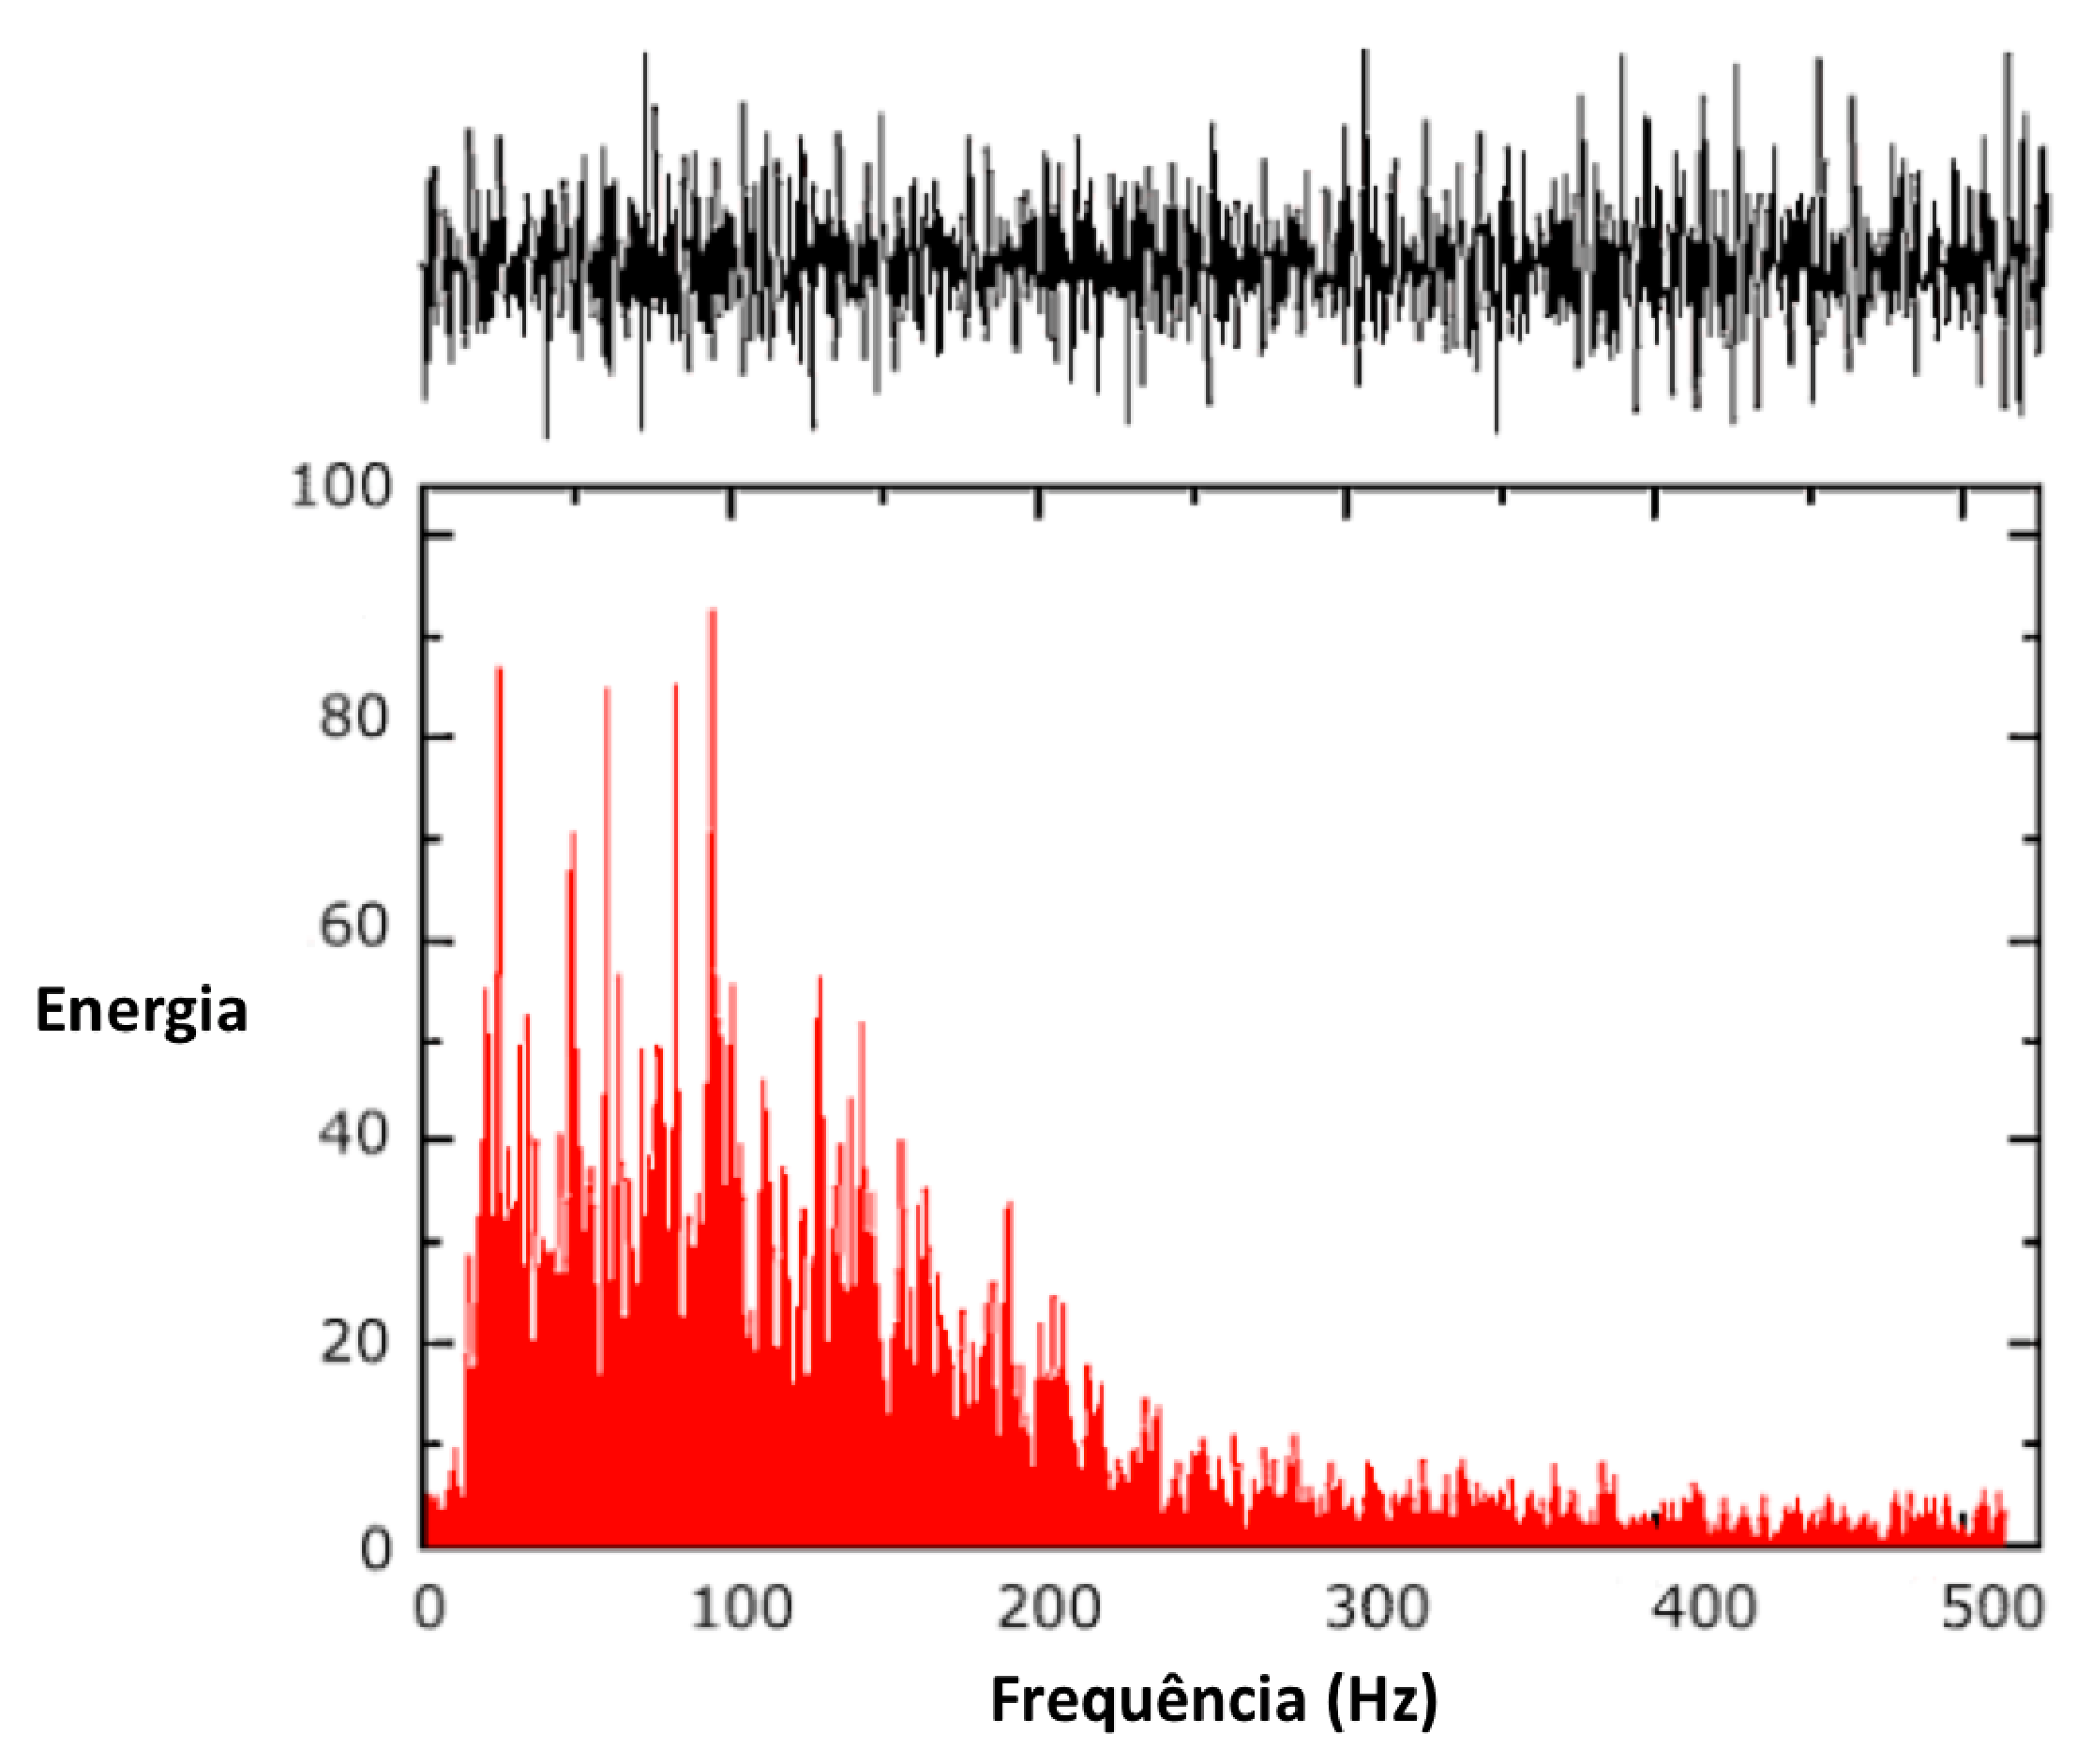
\includegraphics[width=0.6\textwidth]{fig/fft_emg.eps}
	\caption {Sinal do músculo tibial anterior nos domínios do tempo (em preto) e da frequência (em vermelho). Fonte:~\parencite{DELUCA2002}}
  \label{fig:fft_emg}
\end{figure}

Uma das principais preocupações durante a aquisição do sinal mioelétrico é com relação ao ruído presente no sinal. Diversas são as fontes típicas de ruído neste tipo de aplicação, dentre as quais:

\begin{itemize}
  \item \textbf{Ruído proveniente dos  componentes eletrônicos do circuito de aquisição:} todos os componentes eletrônicos geram ruídos que estão contidos em uma ampla faixa de frequência e que não podem ser eliminados completamente, apenas mitigados com a utilização de componentes eletrônicos de boa qualidade, elaboração cuidadosa de projeto de circuito e técnicas de construção adequadas;
  \item \textbf{Ruído ambiente advindo de fontes de radiação eletromagnética:} este tipo de ruído tem origem em lâmpadas, transmissores de rádio e televisão, fios elétricos, etc. Pode ser atenuado com a utilização de caixas metálicas para a proteção dos circuitos de aquisição;
  \item \textbf{Ruído da rede elétrica:} é o ruído de maior predominância no sinal de interesse, causado pela rede elétrica que tem como frequência fundamental $60$~Hz. Esse tipo de ruído pode ser atenuado com o uso de filtros \textit{notch} que são filtros com uma seletividade de banda de frequência muito restrita. 
  \item \textbf{Ruído de artefato de movimento:} trata-se do ruído gerado pelo movimento dos cabos que ligam os eletrodos ao circuito de aquisição e o próprio movimento entre eletrodo e a pele. Esse tipo de ruído pode ser combatido com a utilização de filtros passa-altas.
\end{itemize}
% ======

% ======
\section{Sistema de aquisição desenvolvido}
\label{sec:sist}
A etapa de pré-processamento do sistema de aquisição desenvolvido acompanha o diagrama em blocos apresentado na Figura~\ref{fig:blocogenerico}.

\begin{figure}[h] 
  \centering
  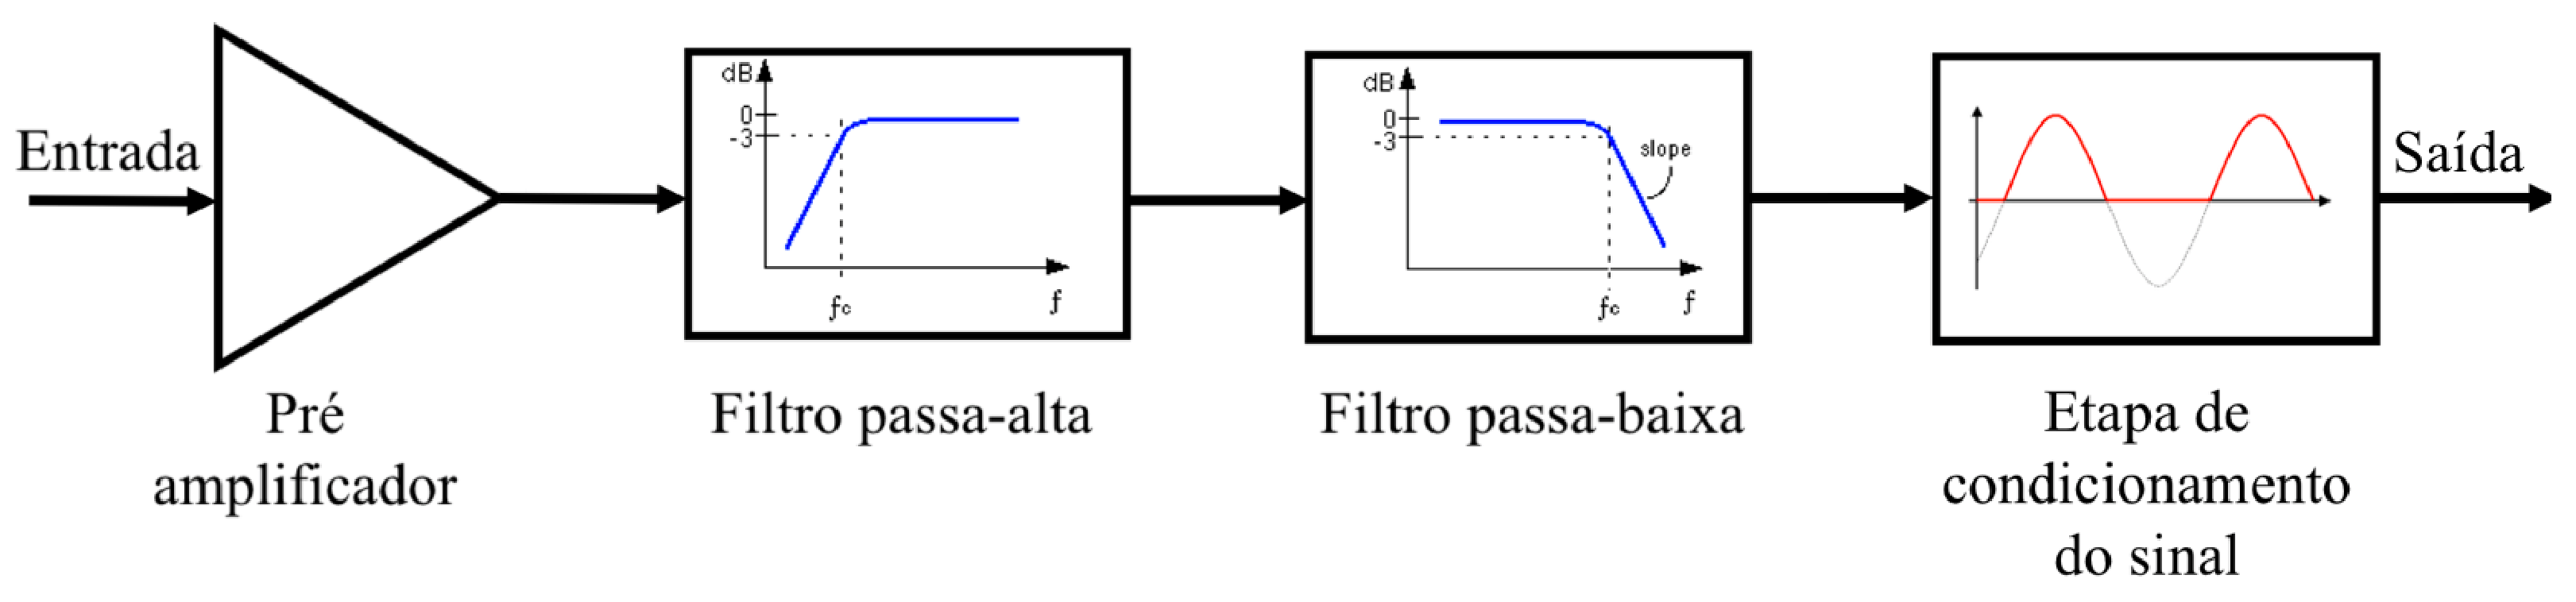
\includegraphics[width=0.6\textwidth]{fig/diagrama_de_blocos_generico}
	\caption{Diagrama em blocos da etapa de pré-processamento. Fonte:~\parencite{limajr2019}.}
  \label{fig:blocogenerico}
\end{figure}

A seguir, cada um dos blocos constituintes da Figura~\ref{fig:blocogenerico} sera visto em maior detalhe.
	
\subsection{Amplificador de instrumentação}
\label{ssec:ampl}
Como primeira etapa do sistema de pré-processamento, temos o amplificador de instrumentação, cuja finalidade elevar a amplitude dos sinais musculares, originalmente na faixa de milivolts, para Volts, atuando também na eliminação de ruídos de modo comum~\parencite{DELUCA2002}. A Figura~\ref{fig:op_amp} mostra um modelo de um amplificador diferencial ideal.
\begin{figure}[h]
  \centering
  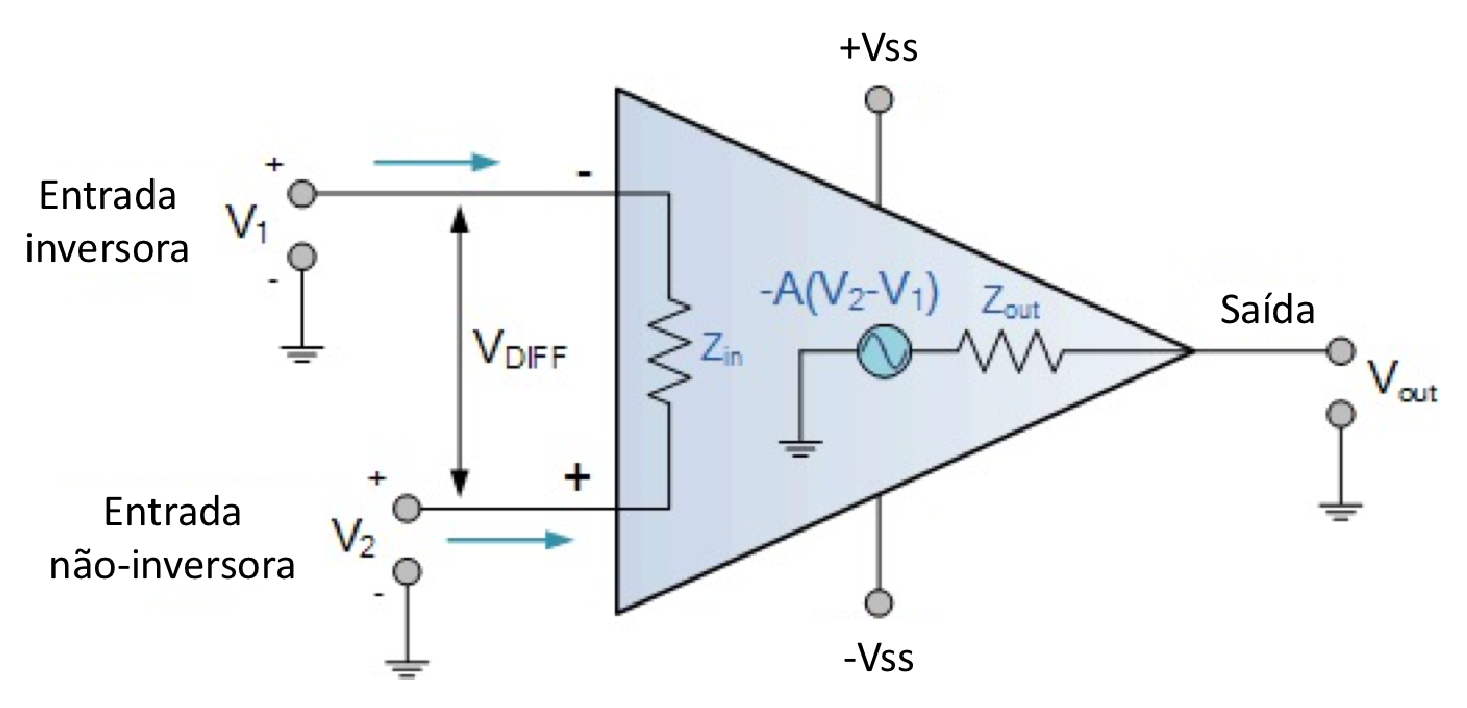
\includegraphics[width=0.6\textwidth]{fig/op_amp}
  \caption{Modelo de um amplificador diferencial ideal. Fonte:~\parencite{ELETRONICS2019}}
  \label{fig:op_amp}
\end{figure}

\subsection{Filtro passa-altas}
\label{ssec:hp}
No sistema desenvolvido optou-se pela topologia \textit{Sallen-Key} por se tratar de uma topologia de baixa complexidade na sua construção e no cálculo de seus componentes. A função de aproximação utilizada é a do filtro \textit{Butterworth}, por ser um dos mais simples e possuir resposta em frequência plana na banda passante~\parencite{BUTTERWORTH}.

A frequência de corte está sintonizada em $10$~Hz com o objetivo de eliminar artefatos de movimento (movimento dos cabos e dos eletrodos de captação do sinal) do sinal mioelétrico.

Foi utilizado um filtro de 1ª ordem, onde um circuito RC é ligado a um amplificador operacional (Figura~\ref{fig:hpf}). 

O cálculo da frequência de corte ($f_c$) é dado por:
     \begin{equation}
     	f_c=\frac{1}{2\pi RC}
     	\label{eq:fc}
     \end{equation}
onde $R$ e $C$ correspondem aos valores de resistência e capacitância no circuito RC em Ohms e Farads, respectivamente.

Fixando os valores de $R= 1,591~M\Omega$ e $C = 10~nF$, tem-se $f_c = 10~Hz$. 

\begin{figure}[h]
		\centering
		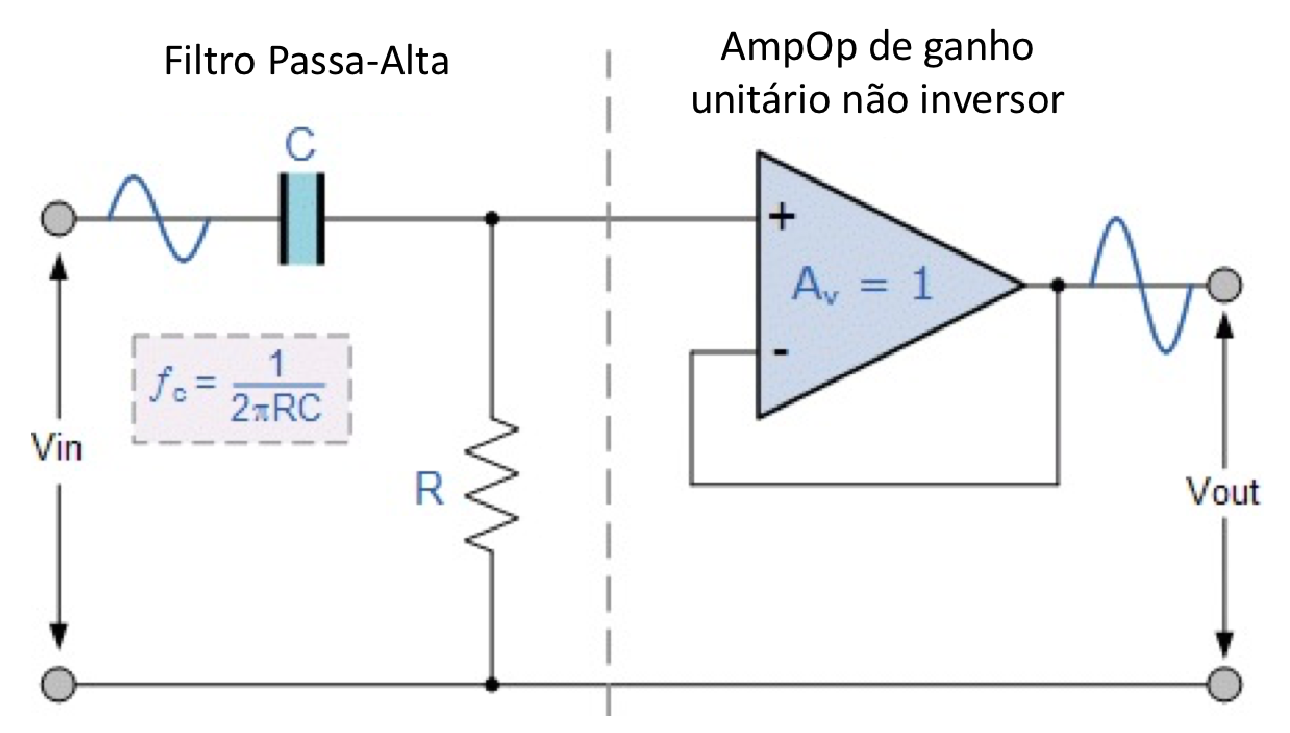
\includegraphics[width=0.6\textwidth]{fig/hpf}
		\caption{Topologia do filtro passa-altas. Fonte:~\parencite{ELETRONICS2019}}
		\label{fig:hpf}
	\end{figure}
     
\subsection{Filtro passa-baixas}      
\label{ssec:lp}
Seguindo a mesma linha de raciocínio do estágio anterior, foi utilizado filtro Butterworth de 2ª ordem e topologia \textit{Sallen-Key}.

A implementação do passa-baixas de 2ª ordem permite maior decaimento do ganho a partir da frequência de corte, $40~dB$ por década, aumentado a seletividade do sistema de pré-processamento em relação à eliminação de altas-frequências. A Figura \ref{fig:lpf} mostra a topologia do filtro passa-baixas utilizado.

	\begin{figure}[h]
		\centering
		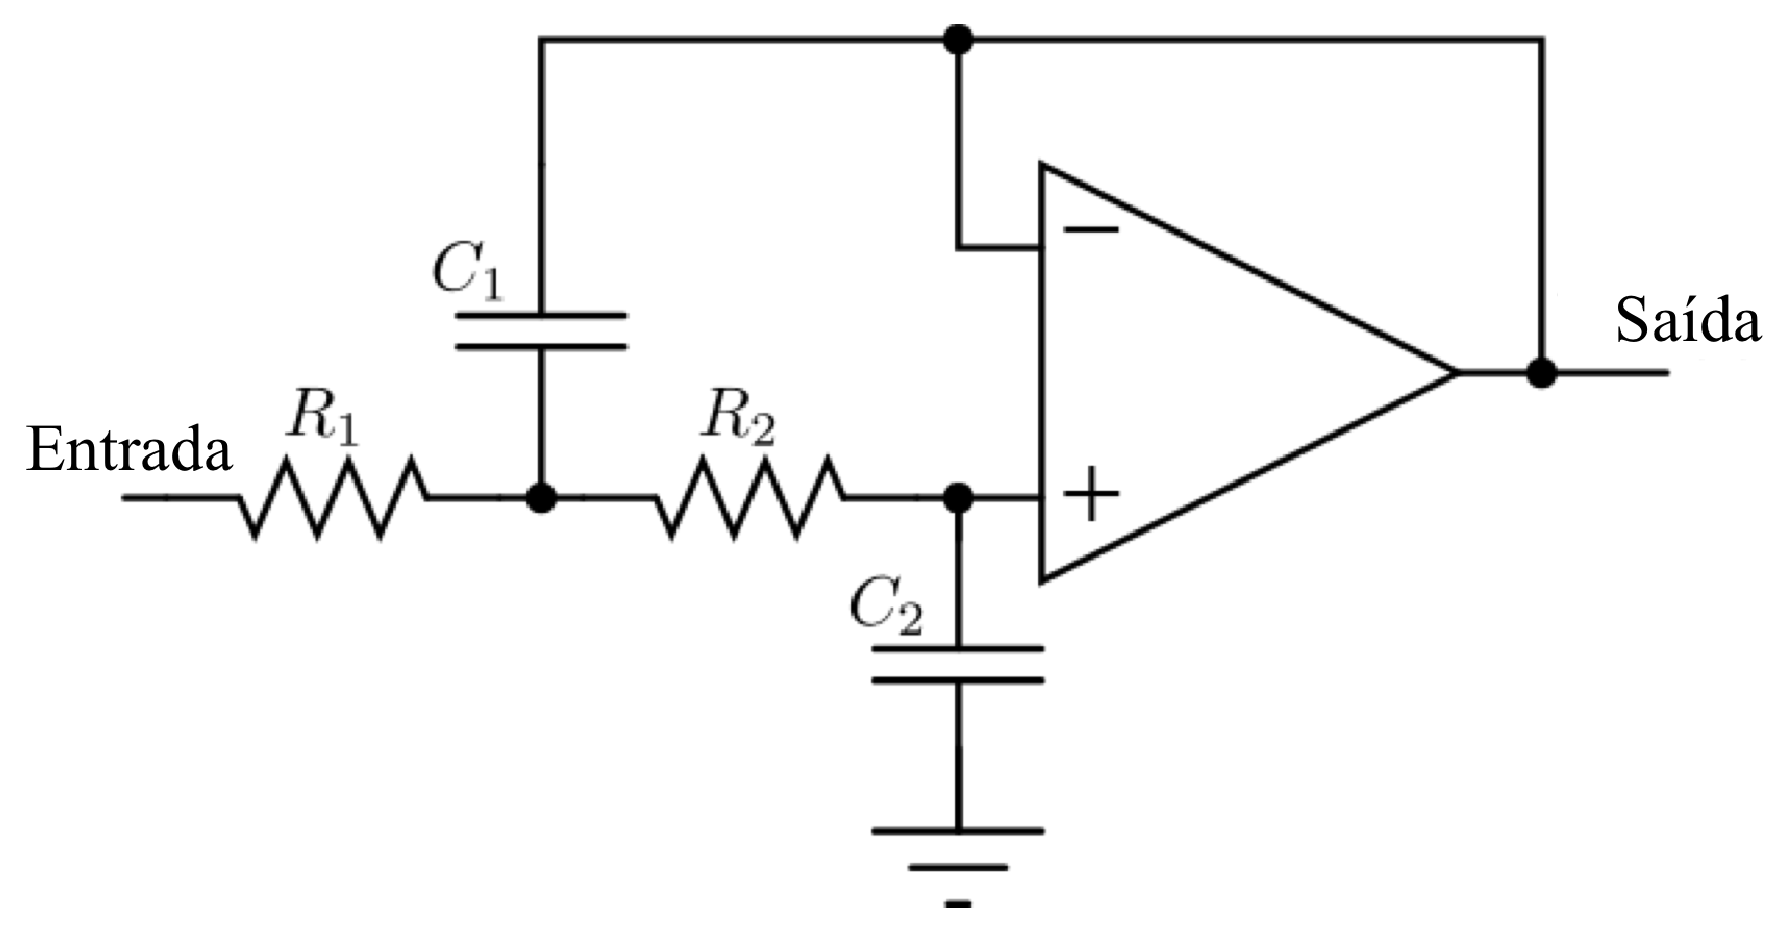
\includegraphics[width=0.6\textwidth]{fig/lpf}
		\caption{Topologia do filtro passa-baixas. Fonte: Wikipédia.}
		\label{fig:lpf}
	\end{figure}

Seguindo a literatura especializada~\parencite{DELUCA2002}, a frequência de corte foi ajustada para $500$~Hz.
 
Para o filtro considerado, a frequência de corte é dada pela expressão:
	\begin{equation}
     	f_c = \frac{1}{2\pi\sqrt{R1 \cdot R2 \cdot C1 \cdot C2}}
     	\label{eq:fcseg}
     \end{equation}

Para haver ganho unitário na banda passante e $f_c = 500$~Hz, escolheu-se  $R_1 = R_2 = 22,5~k\Omega$, $C_1 = 20$~nF e $C_2 = 10$~nF.  


\subsection{Simulação e teste do circuito de pré-processamento}
\label{ssec:simula}	
Nesta implementação, a conversão analógico-digital é realizada por uma placa de áudio (UCA 200, desenvolvida pela~\citeauthor{BEHRINGER2019}), o que permitiu a supressão o bloco \emph{etapa de condicionamento do sinal}. A Figura~\ref{fig:esqsofiltros} mostra o esquemático final do circuito de pré-processamento (entrada de sinais sendo representada pela fonte de tensão V1).
\begin{figure}[h] 
  \centering
  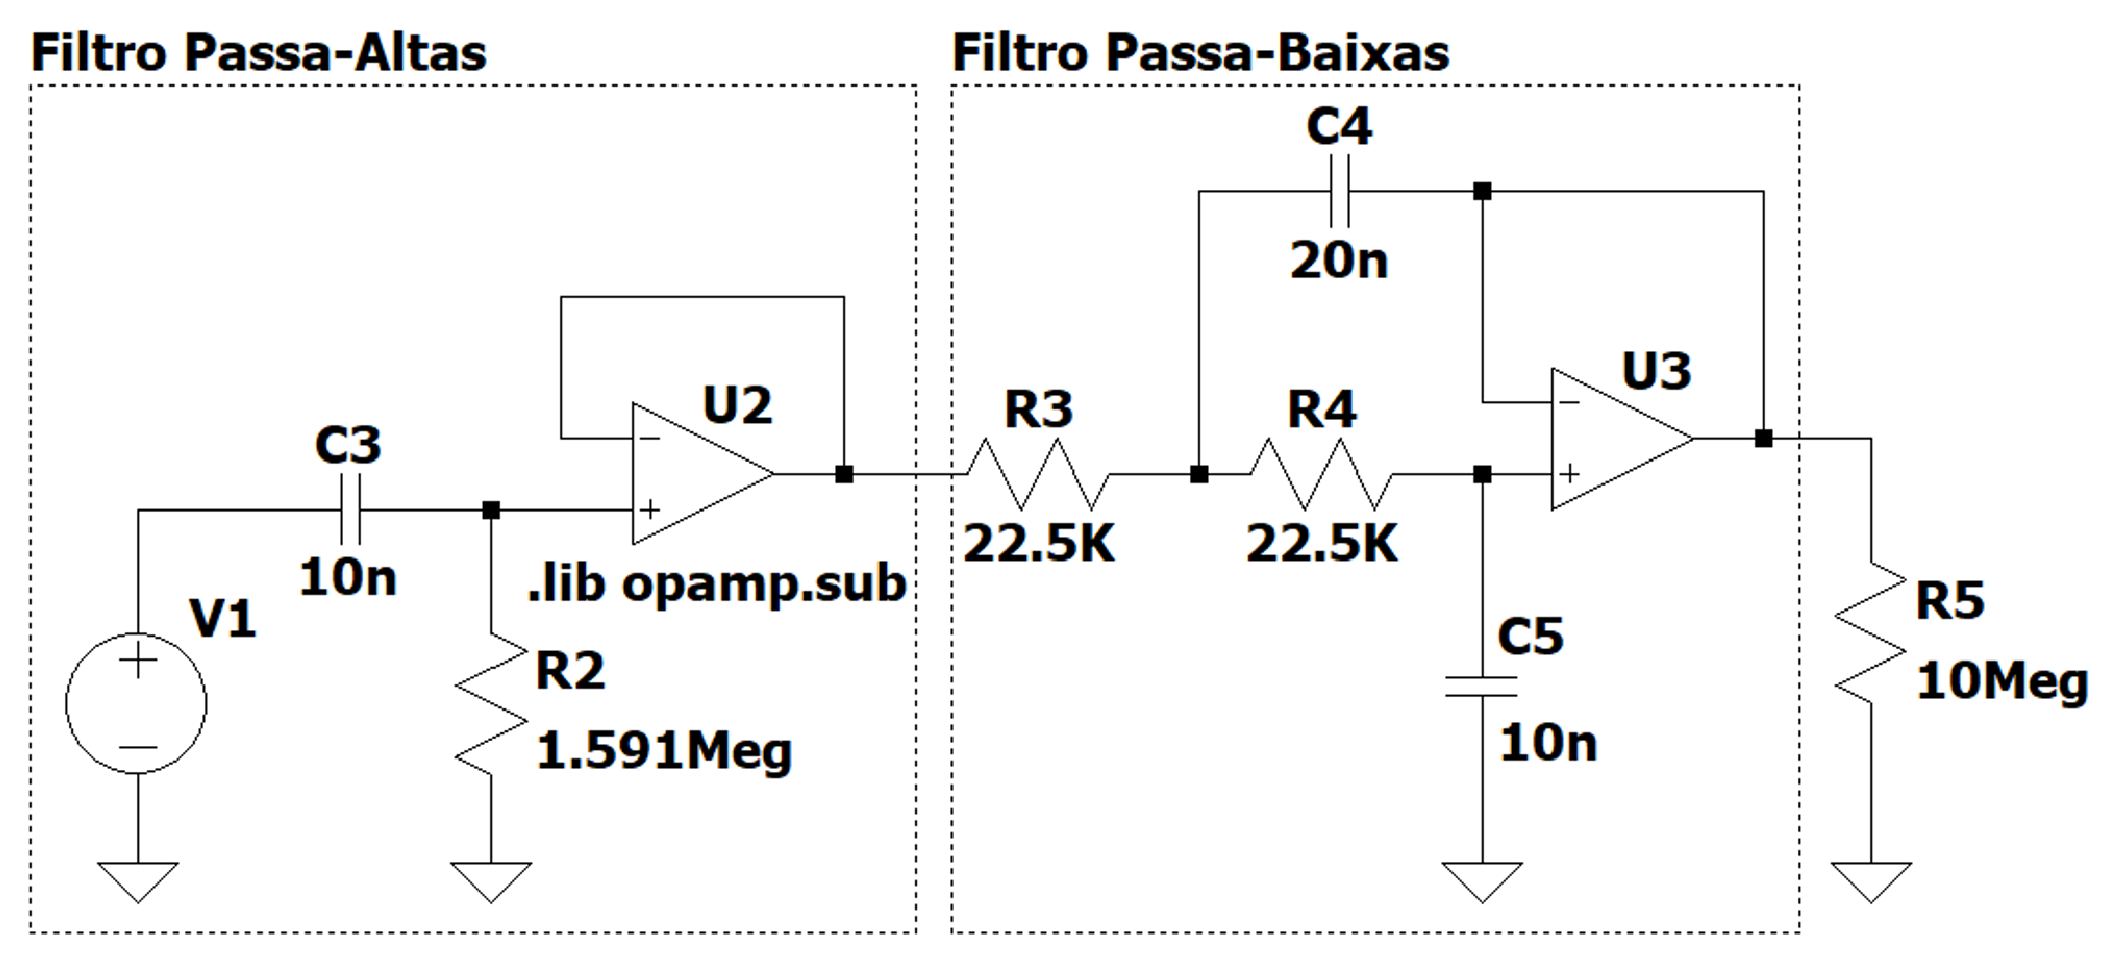
\includegraphics[width=0.6\textwidth]{fig/esquematico_so_filtros}
	\caption{Esquemático do circuito apenas com os filtros. Fonte:~\parencite{limajr2019}.}
  \label{fig:esqsofiltros}
\end{figure} 
	
A Figura~\ref{fig:grafsofiltros} mostra a resposta em frequência do circuito e, como esperávamos, as frequências de corte estão coerentes com o esperado: frequência de corte inferior e superior, respectivamente, iguais a $10$ e $500$~Hz.
\begin{figure}[h] 
  \centering
  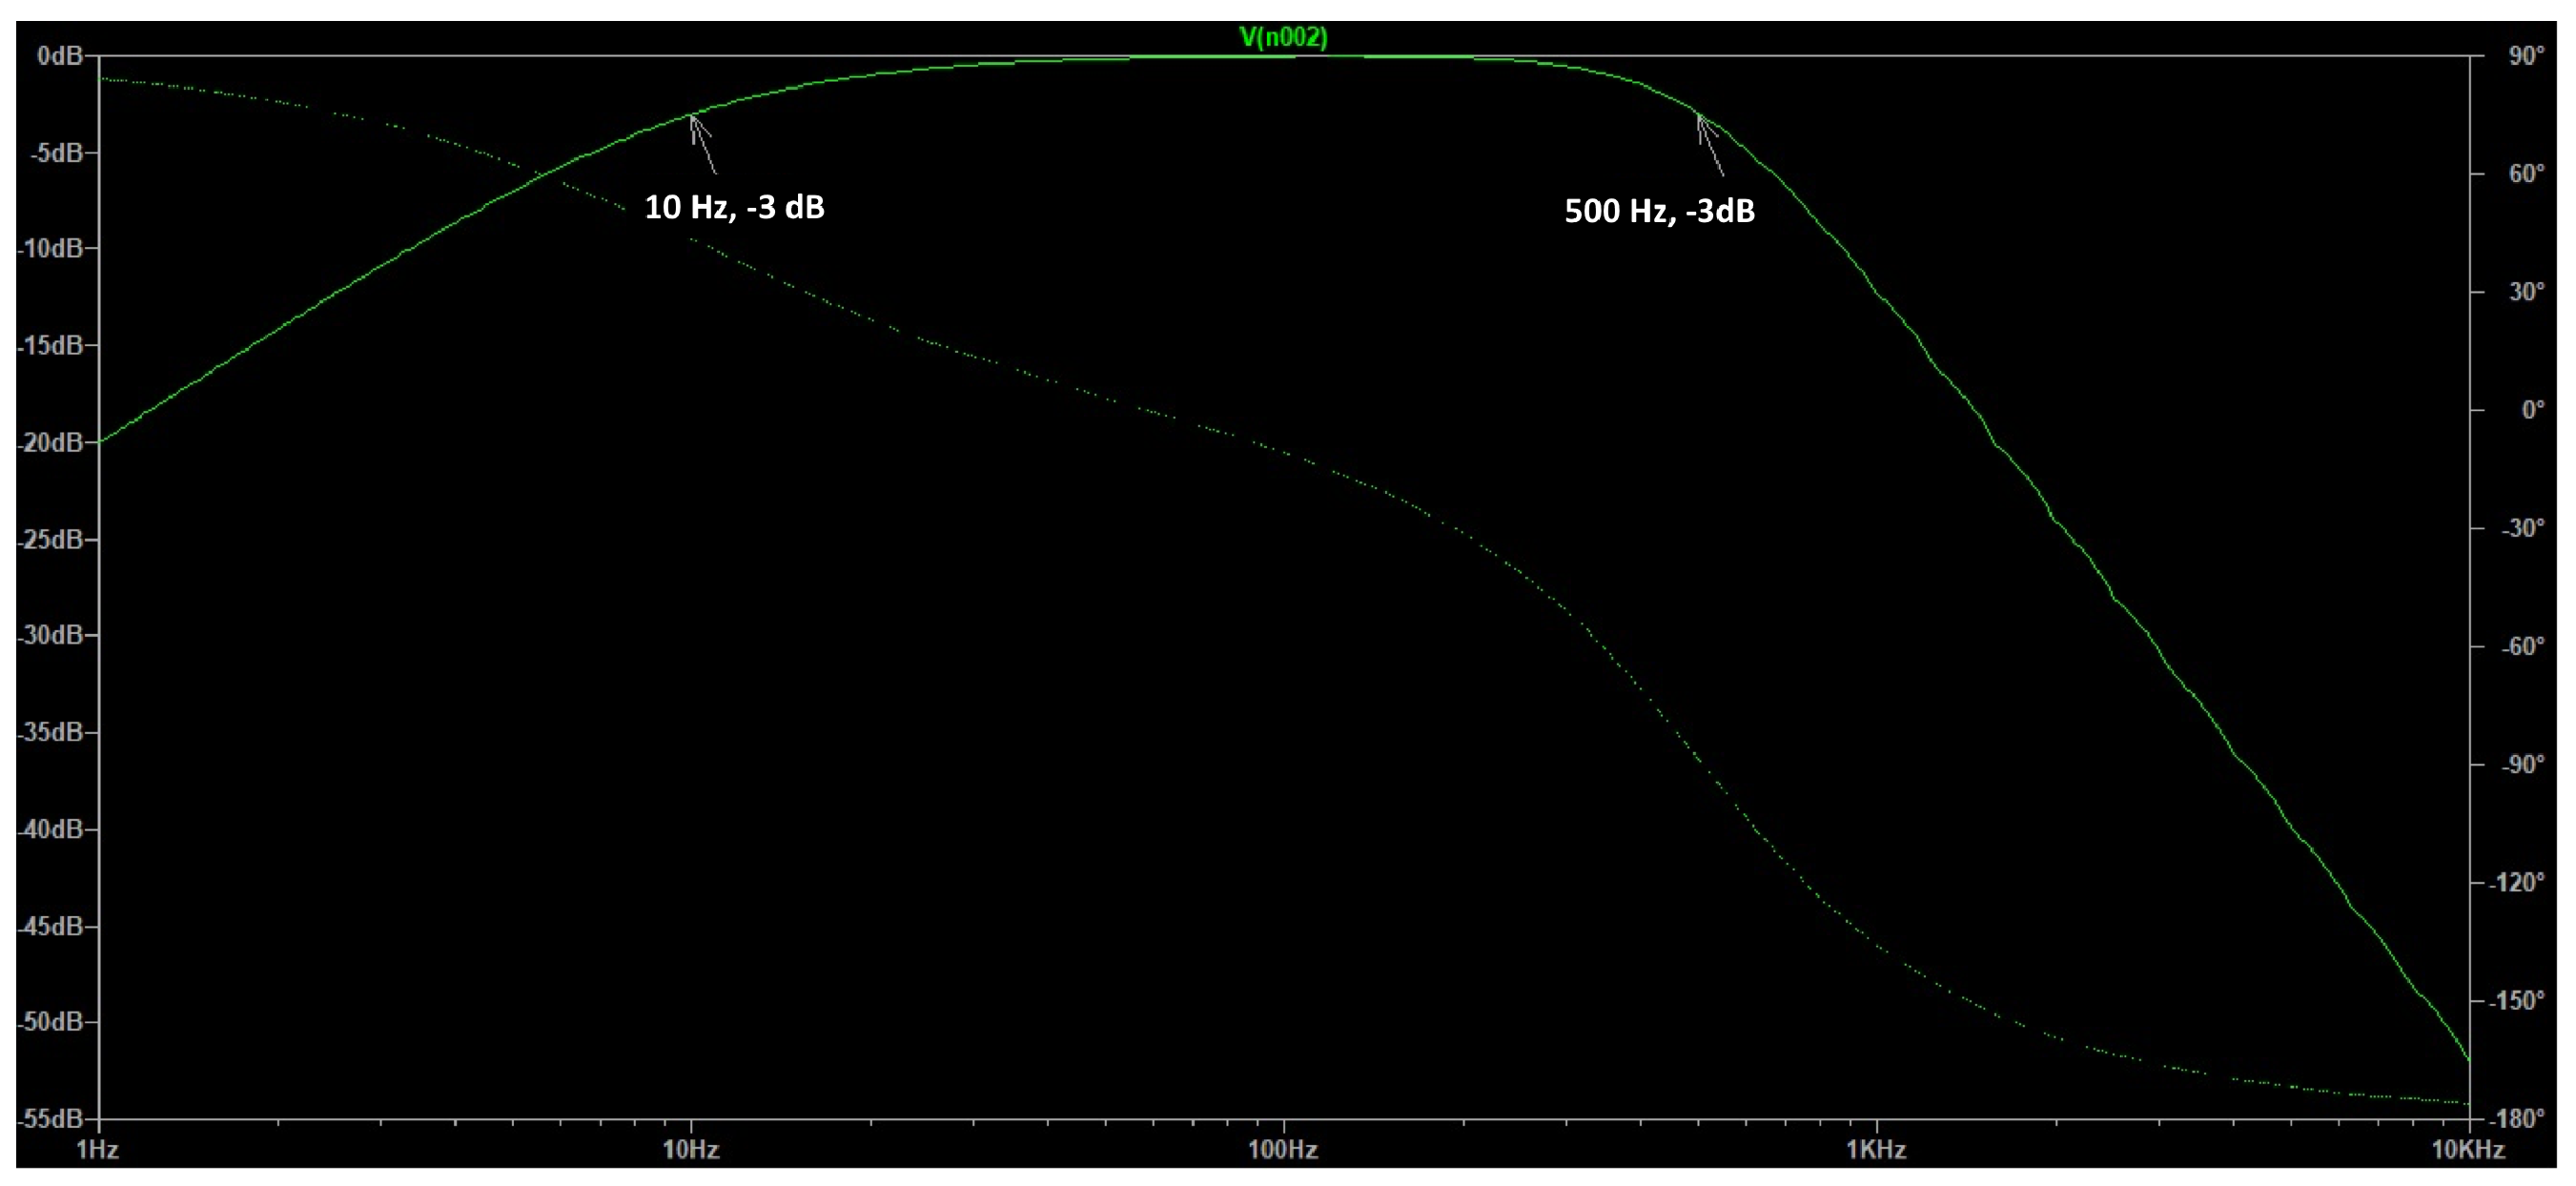
\includegraphics[width=0.6\textwidth]{fig/grafico_so_com_filtros}
	\caption{Gráfico da resposta em frequência do circuito implementado. Fonte:~\parencite{limajr2019}.}
  \label{fig:grafsofiltros}
\end{figure} 
	
Com o intuito de proteção e diminuir as possíveis interferências eletromagnéticas, utilizamos caixas metálicas para a acomodação dos protótipos (Figura~\ref{fig:s0_filtros}).
	\begin{figure} [h]
		\centering
		\includegraphics[width=0.6\textwidth]{fig/caixas}
		\caption{Protótipos acomodados em caixas metálicas. Fonte:~\parencite{limajr2019}.}
		\label{fig:s0_filtros}
	\end{figure}

Na Figura~\ref{fig:sinal_filtros}, apresentamos o setup completo do sistema de aquisição do sinal.

	\begin{figure}[h]
		\centering
		\includegraphics[width=0.8\textwidth]{fig/sinal_filtros}
		\caption{Setup final do sistema de aquisição de sinal. Fonte:~\parencite{limajr2019}.}
		\label{fig:sinal_filtros}
	\end{figure}

A título de exemplo de funcionamento do sistema implementado, foi feita a aquisição de sinal mioelétrico correspondente à atividade muscular na região do flexores do antebraço direito de um indivíduo. Foram utilizados três eletrodos conectados à entrada do circuito de aquisição, onde os dois primeiros foram fixados próximos um ao outro na região dos músculos flexores do antebraço direito e o terceiro, responsável pelo nível de referência, foi fixado na região óssea próxima ao cotovelo.

Os movimentos escolhidos para a aquisição do sinal foram:
	\begin{itemize}
		\item O abrir e fechar da mão;
		\item O movimento de pinças entre polegar-indicador, polegar-médio, polegar-anular e polegar-mínimo
	\end{itemize}
onde o primeiro movimento foi realizado três vezes, com intervalo de um segundo entre cada execução e os movimentos de pinça com intervalos de um segundo entre eles.

Seguem os resultados:
	\begin{figure}[h]
		\centering
		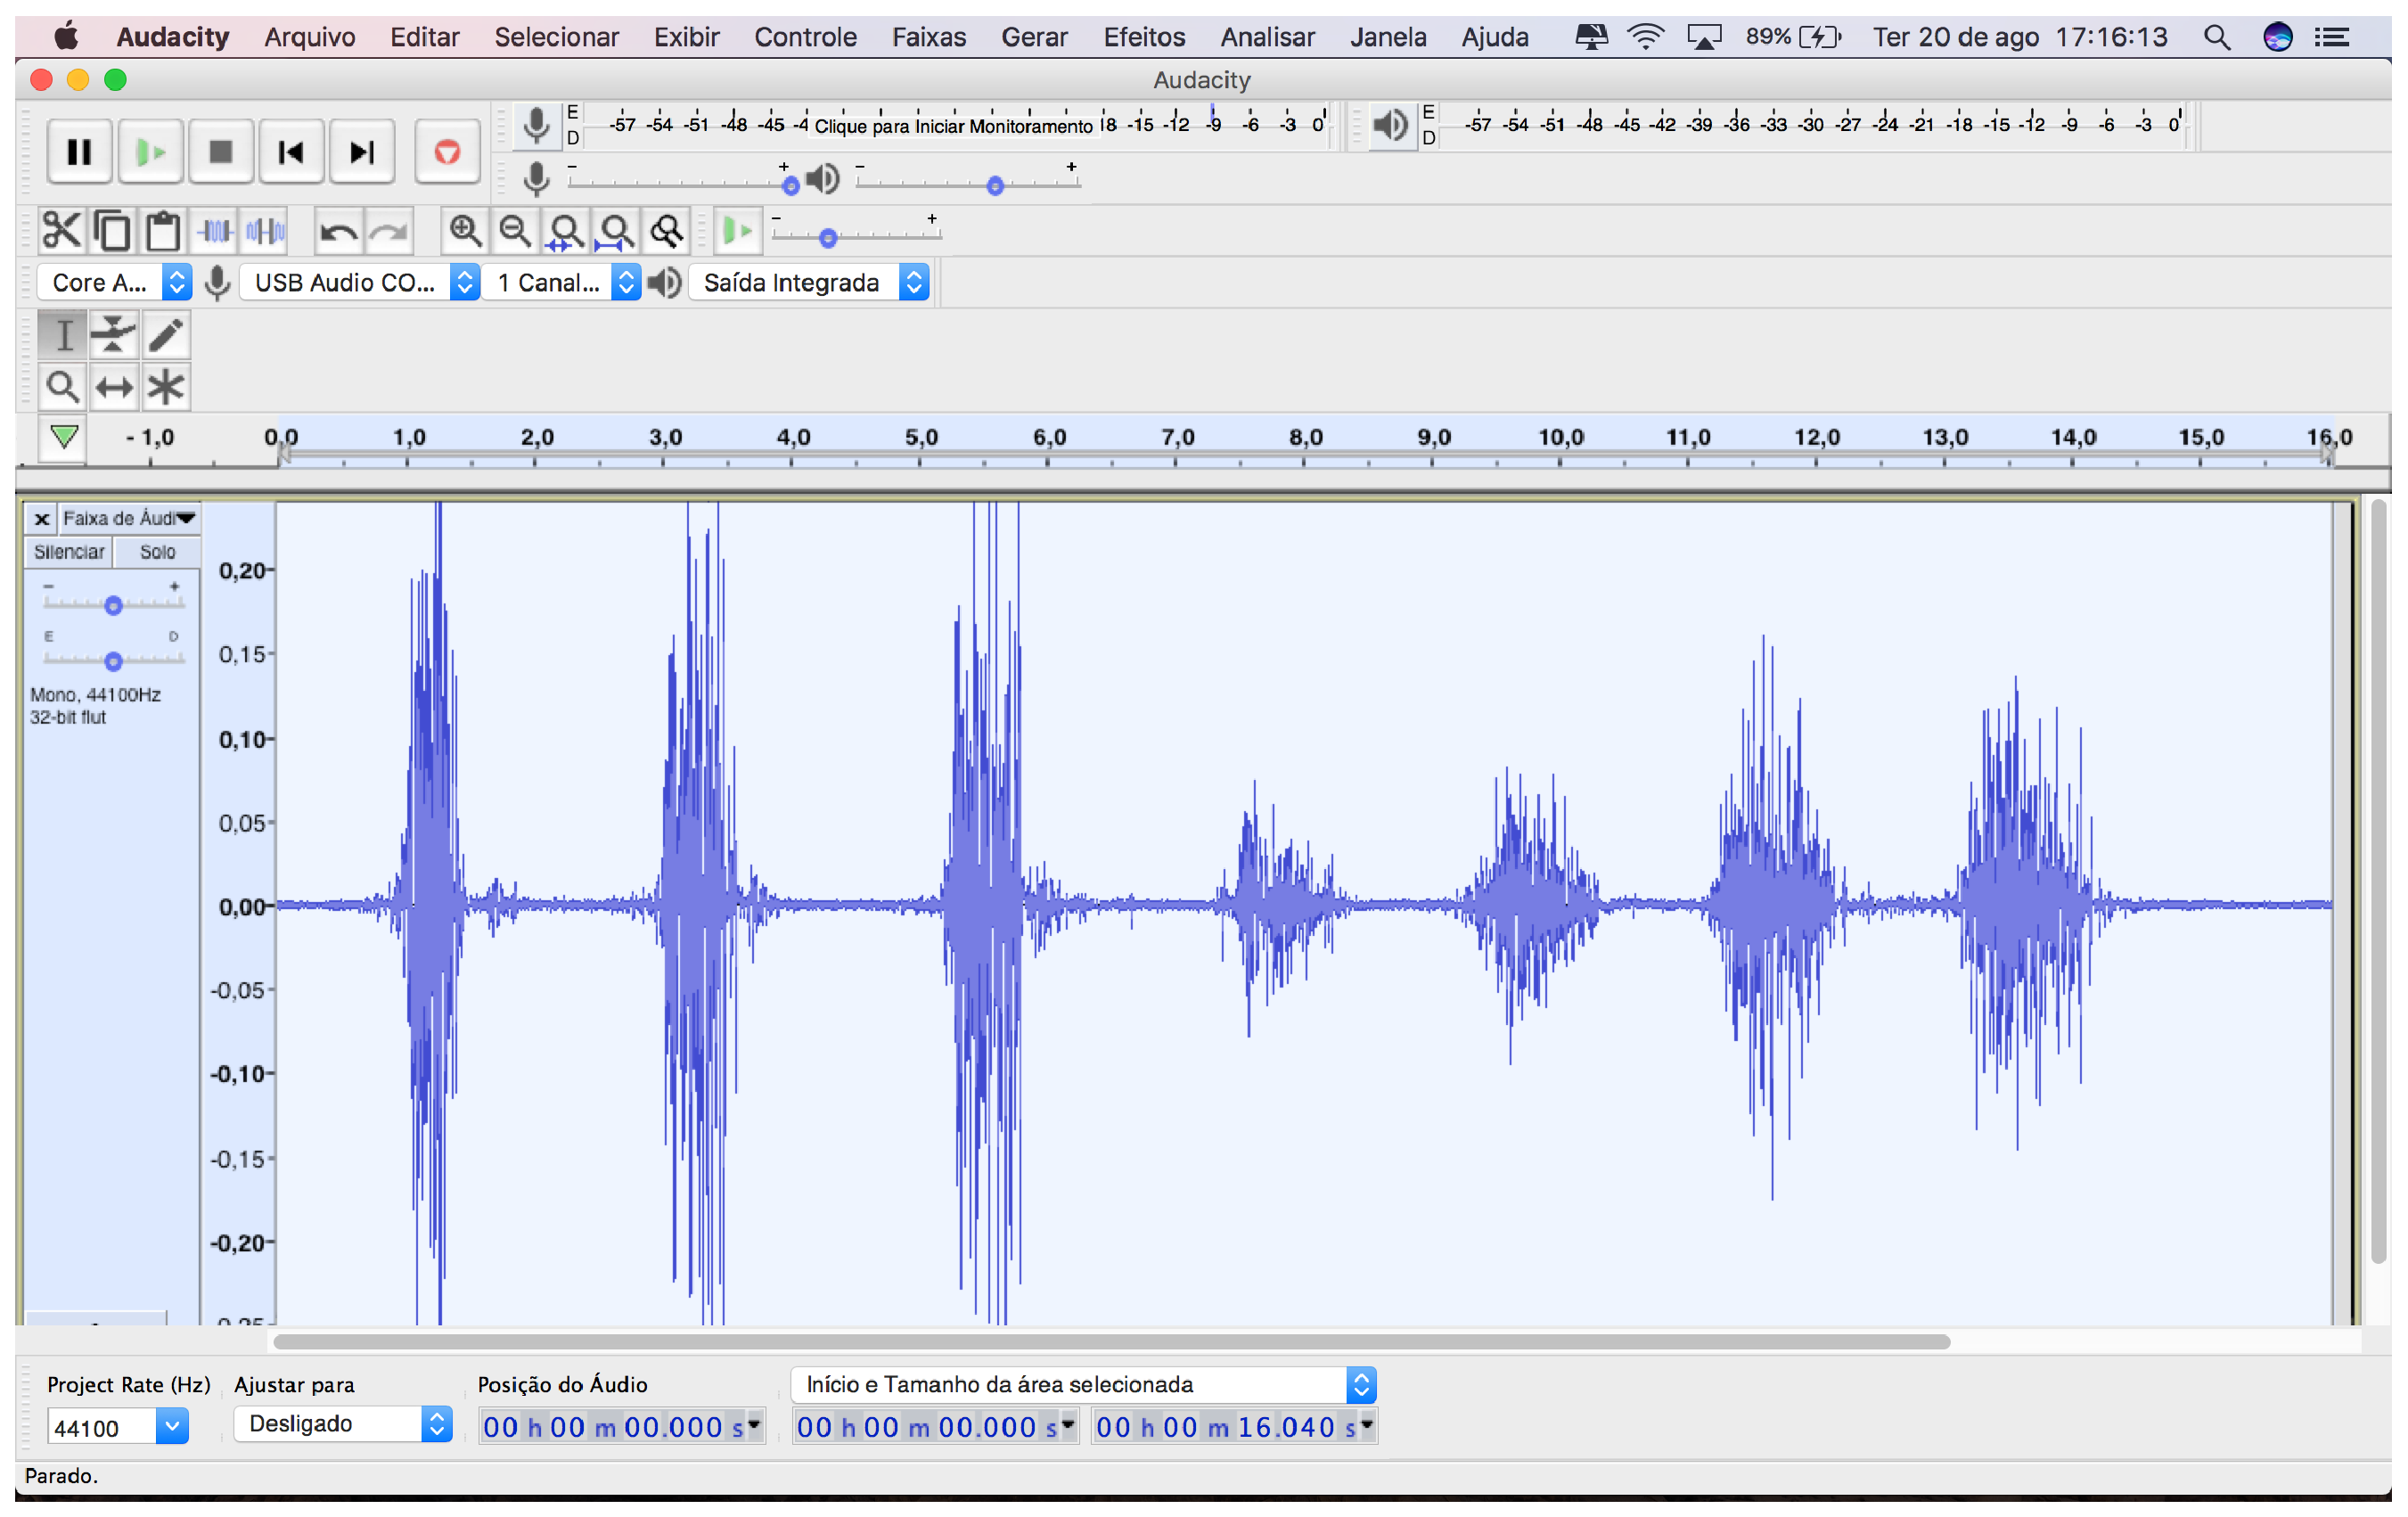
\includegraphics[width=0.8\textwidth]{fig/captura_filtros}
		\caption{Gráficos dos sinais obtidos. Fonte:~\parencite{limajr2019}.}
		\label{fig:captura_ret}
	\end{figure}
	
%\section{Conclusão}
%\label{sec:concl}
 
\printbibliography
\end{document}
